\section{Introduction}
\label{sec:intro}

Organizations adapt large public pretrained models to their own data by
fine-tuning~\paperonly{\cite{hu2022lora}}\tronly{\cite{bommasani2021opportunities,hu2022lora}}. Often several
organizations hold complementary data over the same task, different patient
populations, fraud patterns, or customer bases, and each would obtain an enhanced
model from the combination than from its own data alone~\cite{sheller2020federated}. However, pooling data is challenging because data protection law restricts the sharing of
confidential records across institutions~\paperonly{\cite{gdpr2016}}\tronly{\cite{gdpr2016,hipaa,kvkk2016,pipl2021,dpdp2023}}. \tronly{Competitive concerns
point the same way, and handing the data to whoever operates the fine-tuning
infrastructure raises the same objection~\cite{xiao2023offsite}.} Three obstacles
stand between that setting and a protocol these organizations could deploy.

Federated learning (FL) enables collaboration~\cite{mcmahan2017communication},
and its privacy risk is concentrated at training time~\cite{nasr2019comprehensive,melis2019exploiting}. The protocol exchanges model
updates instead of data, but the updates are themselves vulnerable to privacy attacks. An adversary aggregating a client's per-round
updates can perform membership inference at $25.3\%$ true positive rate at $0.1\%$
false positive rate, against $0.18\%$ from a single snapshot~\cite{zhu2025fedmia}. Two factors therefore determine the attack surface: what a protocol reveals during training and how frequently it is revealed.

\paperonly{Eliminating this surface requires two measures to be taken together. Making the protocol \emph{one-shot}, hence each client contributes only once, ensures that there is no intermediate state for anyone to observe. Encrypting the single
contribution such that the only exchanged value is never available in
plaintext.
In this paper, \emph{one-shot} does not mean that the parties stop communicating. Rather, it means that no intermediate training artifact is ever exposed.
 Prior work applies one of these
measures at a time. One-shot FL~\cite{guha2019oneshot} sends its
single contribution in
plaintext~\paperonly{\cite{zhang2022dense,tang2024fusefl}}\tronly{\cite{zhang2022dense,dai2024coboosting,tang2024fusefl}}, or protects it
with differential privacy (DP)~\cite{hoech2022fedauxfdp}, which
adds noise to the artifact it releases.
 Encrypted FL runs many rounds of
encrypted training or encrypted aggregation, paying the cryptographic cost on
every round, and training under encryption forces polynomial
replacements of every activation and a deep, repeatedly bootstrapped
circuit~\cite{sav2021poseidon}. Thus, adapting a pretrained transformer through this approach is impractical.}

\tronly{Eliminating this surface requires two measures to be taken together. Making the protocol \emph{one-shot}, hence each client contributes only once, ensures that there is no intermediate state for anyone to observe. Encrypting the single
contribution such that the only exchanged value is never available in
plaintext.
In this paper, \emph{one-shot} does not mean that the parties stop communicating. Rather, it means that no intermediate training artifact is ever exposed.
 Prior work applies one of these
measures at a time. One-shot FL~\cite{guha2019oneshot} sends its
single contribution in
plaintext~\paperonly{\cite{zhang2022dense,tang2024fusefl}}\tronly{\cite{zhang2022dense,dai2024coboosting,tang2024fusefl}}, or protects it
with differential privacy~\cite{hoech2022fedauxfdp}, which
adds noise to the artifact it releases.
 Encrypted FL runs many rounds of
encrypted training or encrypted aggregation, paying the cryptographic cost on
every round, and training under encryption forces polynomial
replacements of every activation and a deep, repeatedly bootstrapped
circuit~\cite{sav2021poseidon}. Thus, adapting a pretrained transformer through this approach is impractical.}

Applying both measures still leaves one artifact exposed, namely the model itself.
One-shot protocols end by handing the final model to every participant, which
rules them out when the model may not be distributed at all. A model fine-tuned on
confidential records can be a regulated artifact in high-risk domains such as
health, biometrics, and credit~\cite{euaiact2024}.

In this work, we present HE-OFT, the first one-shot federated fine-tuning protocol
that enables several parties to adapt a pretrained model together and to query the
result, without any of them ever holding it in plaintext. The contribution is encrypted under multiparty
CKKS~\cite{cheon2017ckks,mouchet2021multiparty}, a homomorphic encryption scheme
where secret key is split across the parties.
 The backbone remains public and in plaintext, thus the cryptographic cost does not grow with its size. At no point in the protocol is a training artifact, plaintext contribution, or plaintext model exposed.

\begin{figure*}[t]
\centering
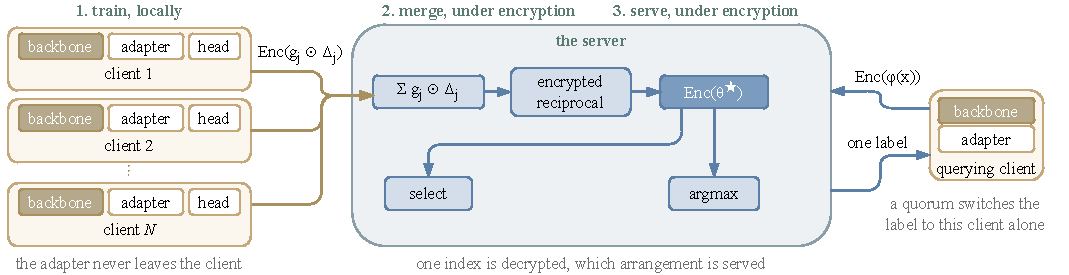
\includegraphics{figures/fig_protocol}
\caption{The protocol in three stages. Each client fine-tunes an adapter and a
classifier head on the same frozen public backbone, keeps the adapter, and
uploads one encrypted head displacement weighted by its per-class counts. The
server adds the ciphertexts and divides by the per-class totals under
encryption, holding no decryption key, so the shared head $\thstar$ exists only
as a ciphertext. The same server answers queries.}
\label{fig:training}
\end{figure*}


\Cref{fig:training} shows how the shared head is built. Every client fine-tunes an
adapter and a classifier head on the same frozen public backbone, keeps the
adapter, and uploads one encrypted head displacement weighted by the classes it
holds. The server adds the ciphertexts and divides by the per-class totals under
encryption, thus the shared head exists only as a ciphertext, and the server does not hold any
key to decrypt it.

The querier must build its query from parts that it can run itself. Therefore, those parts must
be public. The shared trained quantity therefore comes after the last nonlinearity,
which, in a transformer, is a single place. Following this, we summarize our contributions below: 

% \begin{itemize}
% \item \textbf{A split trainable unit.} Each client keeps its own adapter and never
%   transmits it. Only the classifier head is federated, because a client can improve
%   its own features alone but cannot recognize a class it has never seen. No adapter
%   aggregate exists, thus a coalition of all but one client has no sum from which to
%   subtract its own contributions (\cref{sec:split}).

% \item \textbf{A serving path that never decrypts.} The querying client encrypts its
%   own features, thus the server cannot read the query. Only a label leaves the protocol, hence a
%   client cannot collect the per-class scores that would let it solve for the head
%   (\cref{sec:serving}).

% \item \textbf{A selection rule that runs under encryption.} Two arrangements are
%   servable at the same cost: the shared head over each client's own adapter and the
%   shared head over the bare public backbone. The two fail for opposite reasons, the shared head when few clients hold a class and the personal adapter when a client's representation drifts too far. Which failure binds depends on the task and on the partition, therefore the federation must measure both. Each client scoring both on its own held-out data and voting estimates the
%   wrong quantity. The
%   estimator given here corrects that, needs no fitted threshold, and reveals only
%   which arrangement won (\cref{sec:selection}).

% \end{itemize}


\begin{itemize}
\item \textbf{We split the trainable unit.} We federate the classifier head alone.
  Each client keeps its adapter and never transmits it, because a client can improve
  its own features alone but cannot recognize a class it has never seen. The protocol
  forms no adapter aggregate, and a coalition of all but one client therefore has no
  sum from which to subtract its own contributions (\cref{sec:split}).

\item \textbf{We design a serving path that never decrypts.} The querying client
  encrypts its own features, and the server cannot read the query. We return the
  label alone, and a client therefore cannot collect the per-class scores that would
  let it solve for the head (\cref{sec:serving}).

\item \textbf{We select between arrangements under encryption.} Two arrangements are
  servable at the same cost: the shared head over each client's own adapter and the
  shared head over the bare public backbone. The two fail for opposite reasons, the shared head when few clients hold a class and the personal adapter when a client's representation drifts too far. Which failure binds depends on the task and on the partition, and the federation must measure both. We show that the natural rule, each client scoring both arrangements on its own held-out data and voting, estimates the wrong quantity. Our estimator corrects it, needs no fitted threshold, and reveals only which arrangement won (\cref{sec:selection}).

\end{itemize}

\noindent We evaluate HE-OFT on four text classification tasks and one vision task, with
frozen RoBERTa~\cite{liu2019roberta} and vision transformer (ViT)~\cite{dosovitskiy2021vit} backbones, and we implement the cryptographic protocol in
real multiparty CKKS rather than simulating it.
